\documentclass{TIJMUjiaoanLL}
\pagestyle{empty}


\begin{document}


%课程名称
\kecheng{系统生物学}
%课程内容
\neirong{概论\ /\ 第1章}
%教师姓名
\jiaoshi{伊现富}
%职称
\zhicheng{讲师}
%教学日期(格式:XXXX年XX月XX日XX时-XX时)
\riqi{2017年2月20日10:00-12:00}
%授课对象(格式:XXX系XXXX年级XX班(硕/本/专科))
\duixiang{生物医学工程与技术学院2014级生信班(本)}
%听课人数
\renshu{30}
%授课方式
\fangshi{理论讲授}
%学时数
\xueshi{2}
%教材版本
\jiaocai{系统生物学,第1版}


%教案首页
\firstHeader
\maketitle
\thispagestyle{empty}

\mudi{
\begin{itemize}
  \item 掌握系统生物学的学科定义,研究内容,工作流程,研究方法。
  \item 熟悉与系统生物学相关的方法论。
  \item 了解系统生物学的发展历史。
  \item 自学系统生物学的实际应用。
\end{itemize}
}

\fenpei{
\begin{itemize}
  \item (15')引言与导入:通过介绍系统、生命、生物、科学等专业名词的定义,引申出系统科学、生命科学和生物学,为后续系统生物学的介绍作铺垫。
  \item (35')方法论:介绍与系统生物学相关的还原论、科学统一论、机械论、基因决定论和整体论等方法论,为后续系统生物学的介绍作铺垫。
  \item (45')系统生物学:回顾系统生物学的发展历史,介绍系统生物学的学科定义和研究内容,总结系统生物学的工作流程和研究方法,举例说明系统生物学的实际应用。
  \item (5')总结与答疑:总结授课内容中的知识点与技能,解答学生疑问。
\end{itemize}
}

\zhongdian{
\begin{itemize}
  \item 重点:系统生物学的研究内容,工作流程,研究方法。
  \item 难点:系统生物学相关的方法论。
  \item 解决策略:通过实例讲解和比较类比帮助学生理解、记忆。
\end{itemize}
}

\waiyu{
  \vspace*{-10pt}
  \begin{multicols}{2}
    系统(system)

    生物(organism)

    科学(science)

    生物学(biology)

    生物科学(biological sciences)

    生命科学(life sciences)

    还原论(reductionism)

    机械论(mechanism)

    整体观(holism)

    系统生物学(systems biology)

    整合(incorporation)

    干涉(perturbation)
  \end{multicols}
  \vspace*{-10pt}
}

\fuzhu{
\begin{itemize}
  \item 多媒体:系统生物学的发展历史、研究内容、研究方法、应用实例。
  \item 板书:系统生物学的工作流程。
\end{itemize}
}

\sikao{
  \vspace*{-10pt}
  \begin{multicols}{2}
  \begin{itemize}
    \item 系统生物学的学科定义。
    \item 系统生物学的研究内容。
    \item 系统生物学的工作流程。
    \item 系统生物学的研究方法。
  \end{itemize}
  \end{multicols}
  \vspace*{-10pt}
}

\cankao{
\begin{itemize}
  \item 维基百科等网络资源。
\end{itemize}
}

\firstTail


%教案续页
\newpage
\otherHeader

\parpic[fr]{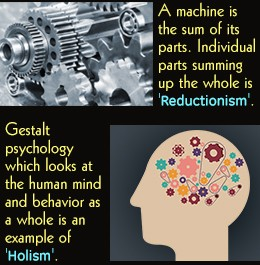
\includegraphics[width=8.4cm]{c1_reductionism_vs_holism_01.jpg}}
\begin{enumerate}
  \item 引言与导入(15分钟)\\
    \textcolor{red}{应用还原论解释系统生物学。}
    \begin{itemize}
      \item 系统生物学 = 系统科学 + 生物科学
        \begin{itemize}
          \item 系统科学 = 系统 + 科学
          \item 生物科学 = 生物 + 科学
        \end{itemize}
      \item 系统生物学 = 系统 + 生物 + 科学
    \end{itemize}

  \item \textcolor{red}{【难点】}方法论(35分钟)
    \begin{itemize}
      \item 还原论:系统 = 部分之和
      \item 机械论:系统 = 机器
      \item 整体论:系统 = 整体
      \item 还原论 vs. 整体论
    \end{itemize}

  \item 系统生物学(45分钟)
    \begin{enumerate}
      \item 发展历史
        \begin{itemize}
          \item Molecular biology $\Rightarrow$ Systems biology
        \end{itemize}
      \item 学科定义\\
        系统生物学是研究一个生物系统中所有组成成分(基因、 mRNA、蛋白质等)的构成,以及在特定条件下这些组分间的相互关系,并通过计算生物学建立一个数学模型来定量描述和预测生物功能、表型和行为的学科。
      \item \textcolor{red}{【重点】}研究内容
\parpic[fr]{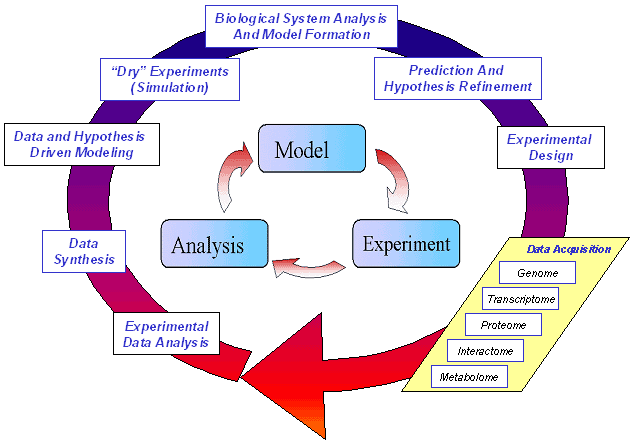
\includegraphics[width=8cm]{c1_sb_workflow_03.png}}
        \begin{itemize}
          \item 湿实验:高通量试验技术,组学研究
          \item 干实验:生物模型,系统仿真
        \end{itemize}
      \item \textcolor{red}{【重点】}工作流程
        \begin{enumerate}
          \item 研究组分,构建模型
          \item 改变条件,观测变化
          \item 比较结果,修订模型
          \item 重新实验,继续修订
        \end{enumerate}
      \item \textcolor{red}{【重点】}研究方法
        \begin{itemize}
          \item 整合 vs. 干涉 
          \item 自下而上 vs. 自下而上
\parpic[fr]{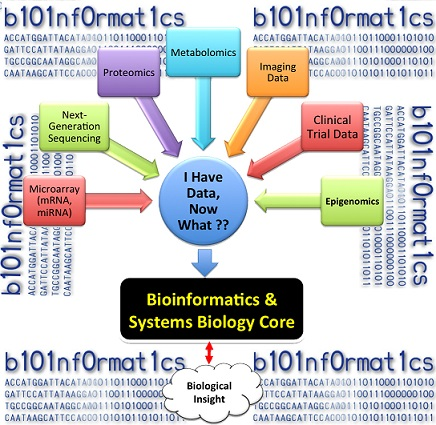
\includegraphics[width=8cm]{c1_sb_future_01.jpg}}
          \item 建模 $\Rightarrow$ 仿真
        \end{itemize}
      \item 应用前景
    \end{enumerate}

% \otherTail
% \newpage
% \otherHeader

  \item 总结与答疑(5分钟)
    \begin{enumerate}
      \item 知识点
	\begin{itemize}
	  \item 系统生物学的学科定义
	  \item 系统生物学的研究内容
	  \item 系统生物学的工作流程
	  \item 系统生物学的研究方法
	\end{itemize}
      \item 技能
	\begin{itemize}
	  \item 方法论与系统生物学
    \item 方法论与实际问题
	\end{itemize}
    \end{enumerate}
\end{enumerate}

\otherTail


\end{document}

